\section{Results}
\label{sec:results}

\subsection{Setup}

All benchmarks ran on an AMD Ryzen 5 7640HS (6 cores, 12 threads), 12\,GiB DDR5, NVMe SSD, Debian 13, \texttt{rustc} 1.94.0 release mode.
Synthetic references of 1\,MB and 10\,MB were generated with ${\sim}40$\% GC content.
Each configuration ran three times with different seeds.
Mean values are reported.

\subsection{Coverage scaling}

Figure~\ref{fig:cov-scaling} shows wall time and peak memory as a function of coverage depth on the 1\,MB reference with 100 mutations.
Both scale linearly ($R^2 > 0.999$).
Throughput stabilises at ${\sim}28{,}000$ read pairs/s above 10x.
The lower rate at 1x reflects startup overhead.

\begin{figure}[t]
  \centering
  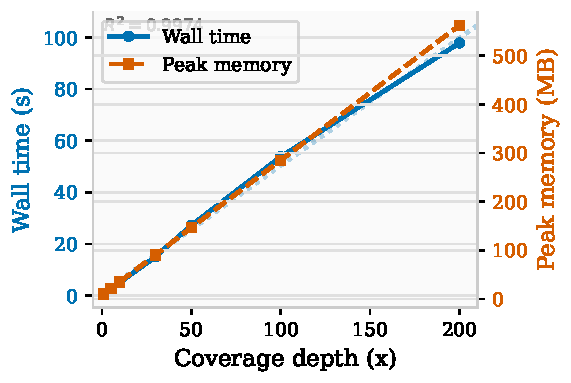
\includegraphics[width=\linewidth]{../../benchmarking/results/graphs/coverage_scaling.pdf}
  \caption{Wall time and peak memory vs coverage depth (1\,MB reference, 100 mutations, 12 threads). Both scale linearly with $R^2 > 0.999$.}
  \label{fig:cov-scaling}
\end{figure}

\subsection{Feature overhead}

Figure~\ref{fig:features} shows the incremental cost of each feature at 30x on the 1\,MB reference (${\sim}200$K read pairs).
Variant injection (+3\%) and GC bias (+2\%) are within noise.
FFPE/oxoG artefacts add 16\% via a per-base damage pass.
UMI simulation dominates at +64\% due to PCR family tracking.
The combined overhead of 125\% is slightly super-additive because UMI families must carry variant and artefact state through each PCR cycle.

\begin{figure}[t]
  \centering
  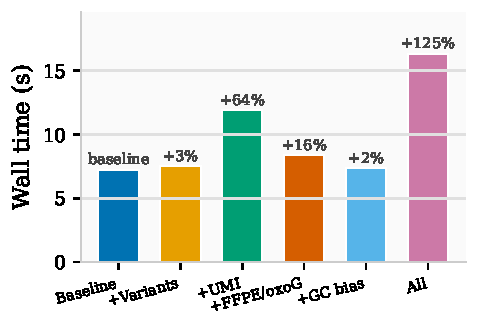
\includegraphics[width=\linewidth]{../../benchmarking/results/graphs/feature_overhead.pdf}
  \caption{Feature overhead relative to baseline (1\,MB, 30x). Variant injection and GC bias are free. FFPE adds 16\%. UMI dominates at +64\%.}
  \label{fig:features}
\end{figure}

\subsection{Throughput}

Table~\ref{tab:scenarios} summarises the main scenarios.
At baseline (10\,MB, 30x, 12 threads), \varforge{} produces ${\sim}1.26$M read pairs in 75\,s (${\sim}13{,}400$ pairs/s, ${\sim}4.0$\,Gbp/min).
Adding 500 mutations increases wall time by $<1\%$.
Figure~\ref{fig:throughput} compares throughput across scenarios.

\begin{table}[t]
\centering
\caption{Main benchmark scenarios (12 threads, mean of 3 runs).}
\label{tab:scenarios}
\small
\setlength{\tabcolsep}{3.5pt}
\begin{tabular}{@{}llrrlrr@{}}
\toprule
Config & Ref & Cov & Var. & Features & Wall (s) & \makecell{Peak\\RAM (GB)} \\
\midrule
Baseline         & 10\,MB & 30x  & ---  & ---             & 75.4  & 3.4 \\
+Variants        & 10\,MB & 30x  & 500  & ---             & 75.9  & 3.4 \\
High coverage    & 10\,MB & 100x & 500  & ---             & 251.1 & 11.1 \\
High cov (1\,MB) & 1\,MB  & 200x & 100  & ---             & 47.8  & 2.2 \\
cfDNA            & 1\,MB  & 200x & 200  & cfDNA, 2\% pur. & 47.5  & 2.3 \\
FFPE + oxoG      & 10\,MB & 30x  & 500  & artefacts       & 87.5  & 4.4 \\
Panel + UMI      & 1\,MB  & 200x & 50   & UMI simplex     & 76.8  & 7.0 \\
\bottomrule
\end{tabular}
\end{table}

\begin{figure}[t]
  \centering
  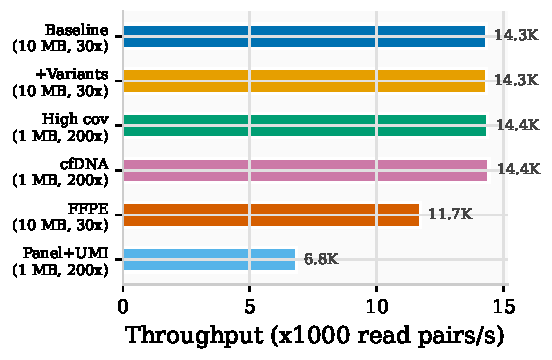
\includegraphics[width=\linewidth]{../../benchmarking/results/graphs/throughput_scenarios.pdf}
  \caption{Throughput across scenarios. Compute-bound configs (1\,MB reference) reach ${\sim}28$K pairs/s. I/O-bound configs (10\,MB) converge to ${\sim}13$--$14$K pairs/s.}
  \label{fig:throughput}
\end{figure}

\subsection{Thread scaling}

Figure~\ref{fig:threads} shows scaling on the 10\,MB, 30x configuration.
Speedup plateaus at 1.16x above 2 threads, indicating I/O saturation from writing ${\sim}280$\,MB compressed FASTQ.
Compute-bound workloads (higher coverage, more features) would scale better.

\begin{figure}[t]
  \centering
  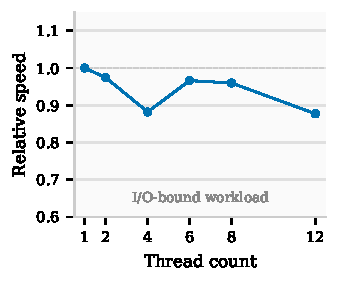
\includegraphics[width=0.75\linewidth]{../../benchmarking/results/graphs/thread_scaling.pdf}
  \caption{Thread scaling (10\,MB, 30x, 500 variants). The plateau at ${\sim}1.16$x reflects FASTQ compression saturating the storage pipeline.}
  \label{fig:threads}
\end{figure}

\subsection{Memory efficiency}

Figure~\ref{fig:mem} shows per-pair memory is constant at ${\sim}1.7$\,KB across coverage depths.
The streaming architecture bounds peak memory to $\text{buffer\_depth} \times \text{batch\_size}$ regardless of dataset size.
With 64 channel slots, the theoretical ceiling is ${\sim}10.5$\,GiB.
A full human genome 30x WGS run (${\sim}600$M pairs) is feasible on a standard workstation.

\begin{figure}[t]
  \centering
  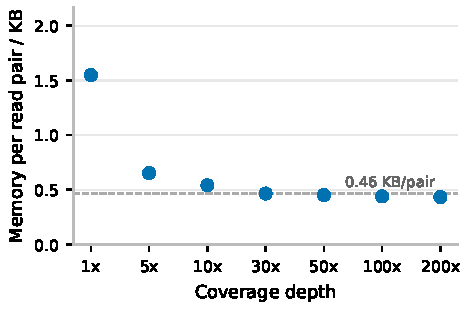
\includegraphics[width=\linewidth]{../../benchmarking/results/graphs/memory_per_pair.pdf}
  \caption{Memory per read pair across coverage depths. The constant ${\sim}1.7$\,KB/pair confirms the streaming architecture bounds memory by batch size, not dataset size.}
  \label{fig:mem}
\end{figure}
